\section{Задание №4}

\begin{enumerate}
        \item Построить датчик распределения Коши.
        \item На основе датчика распределения Коши с помощью метода фон Неймана построить датчик стандартного нормального распределения. При помощи функции \texttt{normal probability plot} убедиться в корректности работы построенного датчика и обосновать наблюдаемую линейную зависимость.
        \item Сравнить скорость моделирования стандартного нормального распределения в заданиях 3 и 4.
\end{enumerate}


\subsection{Построение датчика распределения Коши}

\begin{definition}
        Будем говорить, что случайная величина $X$ \textit{имеет распределение Коши с параметрами $a$ и $b$}, если ее функция распределения имеет вид:
$$
        F_X(x) = \frac{1}{\pi}\arctg\left(\frac{x-a}{b}\right) + \frac{1}{2}.
$$ 
        Будем обозначать такие случайные величины
$$
        X \sim \mbox{C}(a,\,b).
$$
\end{definition}

Функция распределения Коши имеет обратную, поэтому воспользовавшись методом обратной функции распределения (смотри теорему \ref{th:inv-method}), получим
$$
        X = F_X^{-1}(\xi) = a + b \tg\left[\pi(\xi - \nicefrac{1}{2})\right],
        \quad
        \mbox{где } \xi \sim \mbox{U}[0,\,1].
$$


\subsection{Построение датчика стандартного нормального распределения методом фон Неймана}

Метод фон Неймана заключается в моделировании нормального распределения путем мажорирования плотностью распределения Коши с параметрами $a$ и $b$. Для достижения наилучшей оценки, будем подбирать значения параметров $a$ и $b$. Выпишем плотности стандартного нормального распределения и распределения Коши:
$$
        \rho_N(x) = \frac{1}{\sqrt{2\pi}} e^{-\frac{x^2}{2}},
$$
$$
        \rho_C(x) = \frac{1}{\pi}\cdot\frac{b}{(x-a)^2+b^2}.
$$
При моделировании будем использовать следующий алгоритм:
\begin{enumerate}
        \item возьмем некоторое число $k > 0$ такое, что $\rho_N(x) \leqslant k \rho_C(x)$ $\forall x \in \R$;
        \item рассмотрим значение случайной величины $\hat\xi = \xi$, где $\xi \sim \mbox{C}(a,\,b)$;
        \item сгенерируем случайную величину $\hat\eta = \eta$, где $\eta \sim \mbox{Bern}\left(\frac{\rho_N(\hat\xi)}{k\rho_C(\hat\xi)}\right)$;
        \item если $\hat\eta = 1$, то $\hat\xi$ является значением случайной величины из распределения с плотностью $\rho_N(x)$, иначе, продолжаем моделирование, начиная с пункта 2.
\end{enumerate}

Данный алгоритм работает тем быстрее, чем ближе отношение $\frac{\rho_N(x)}{k\rho_C(x)}$ к единице, поэтому в качестве $k$ возьмем $k^* = \min\limits_{a,\,b}\max\limits_{x}\frac{\rho_N(x)}{\rho_C(x)}$. Рассмотрим это отношение:
$$
        \frac{\rho_N(x)}{\rho_C(x)}
        =
        \frac{\sqrt{\pi}}{b\sqrt{2}}
        \cdot
        e^{-\frac{x^2}{2}}
        \cdot
        [(x - a)^2 + b^2].
$$



\clearpage
\begin{figure}[t]
        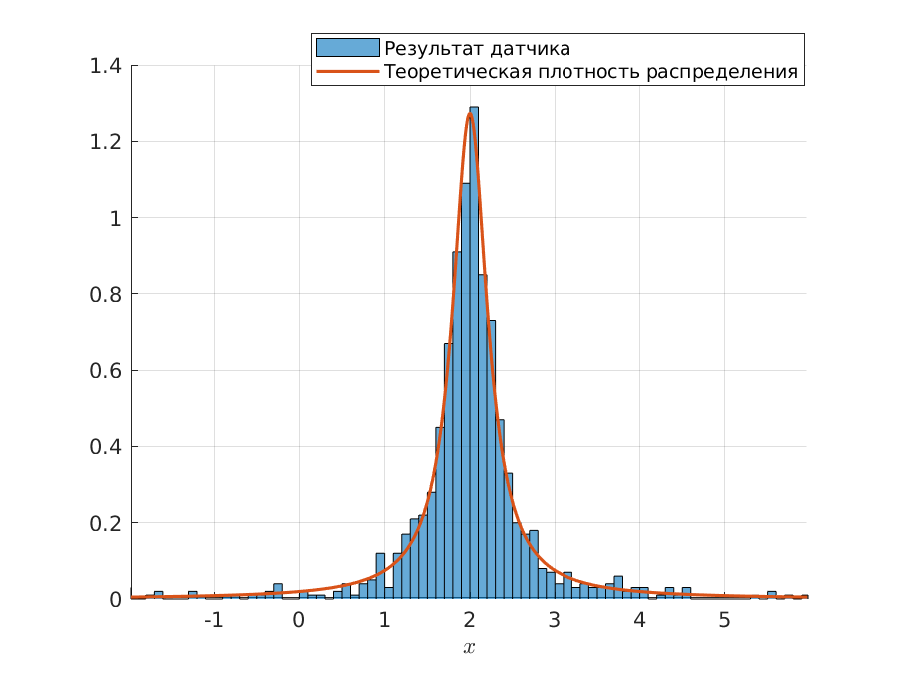
\includegraphics[width=0.5\linewidth]{task_04/c2-025-1000.eps}
        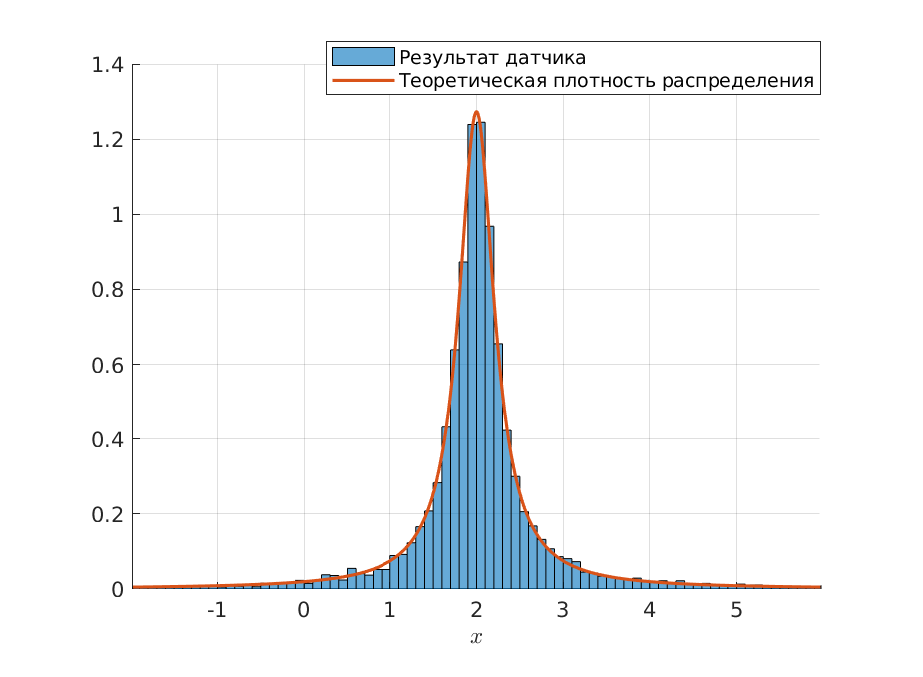
\includegraphics[width=0.5\linewidth]{task_04/c2-025-10000.eps}
        \caption{Гистограмма распределения Коши случайной величины с параметрами $a = 2$ и $b = \nicefrac{1}{4}$ при $10^3$~(слева) и $10^4$~(справа) испытаний.}
\end{figure}